\begin{figure}[H]
    \centering
    \includegraphics[width=.9\linewidth]{al_algo}
    \captionsetup{singlelinecheck=off}
    \caption[]{The algorithm tries to find to a given transmission spectrum the kind of two layer meta surface stack which can reproduce this target. The input spectrum is passed to a convolutional neural network which outputs its guess for the stack and layer parameters. The Database module looks at the two sets of layer parameters and interpolates between stored $S$-matrices to give an estimate for the two $S$-matrices describing the two layers. The SASA algorithm calculates the resulting current transmission spectrum and passes it to the optimizer. This last module compares it to the target spectrum and adjusts the continuous parameters to minimize the difference between the two. Find the details to all parts of the algorithm in the sections below.
    \vspace{1cm}

    \begin{tabular}{ll}
        \vspace{0.8cm}
        \hyperref[sec:NN]{NN}: &
        \begin{tabular}[t]{@{}l@{}}
            convolutional neural network trained to map spectra to stack and \\ layer parameters
        \end{tabular}\\
        %
        \vspace{0.8cm}
        \hyperref[sec:DB]{DB}: &
        database of FMM simulated single layers\\
        %
        \vspace{0.8cm}
        SASA: &
        algorithm calculating $\hat{S}_\s{stack} = \hat{S}_\s{stack}(\hat{S}_1, \, \hat{S}_2, \, \varphi, \, h)$\\
        %
        \vspace{0.8cm}
        \hyperref[sec:opt]{Opt}: &
        \begin{tabular}[t]{@{}l@{}}
            optimizer changing parameters to minimize the difference between\\ the current and target spectrum
        \end{tabular}\\
        %
        \vspace{0.8cm}
        $\hat{S}_1, \, \hat{S}_2$ &
        S-matrices of the top and bottom layer\\
        %
        \vspace{0.8cm}
        layer params &
        \begin{tabular}[t]{@{}l@{}l@{}}
            two sets of continuous parameters:
            $p = (w, \, l, \, t, \, \Lambda)$
            and \\
            discrete parameters: $m \in$ (Al, Au), $g \in$ (rectangles, rectangular holes) \\
            $w$...width, $l$...length, $t$...thickness, $\Lambda$...Period,
            $m$...material, $g$...geometry
        \end{tabular}\\
        %
        \vspace{0.8cm}
        new params &
        \begin{tabular}[t]{@{}l@{}}
            the Opt. only changes the continuous parameters, the discrete ones, \\ e.g. material, remain unchanged
        \end{tabular}\\
        %
        \vspace{0.8cm}
        optimization loop & this loop is repeated until the target accuracy is reached\\
    \end{tabular}
    }
    \label{fig:al:algo}
\end{figure}
